% *********************************************************************
% © 2010–2022 Jeremy Sylvestre
%
% Permission is granted to copy, distribute and/or modify this document
% under the terms of the GNU Free Documentation License, Version 1.3 or
% any later version published by the Free Software Foundation; with no
% Invariant Sections, no Front-Cover Texts, and no Back-Cover Texts. A
% copy of the license is included in the appendix entitled “GNU Free
% Documentation License” that appears in the output document of this
% PreTeXt source code. All trademarks™ are the registered® marks of
% their respective owners.
%
% *********************************************************************

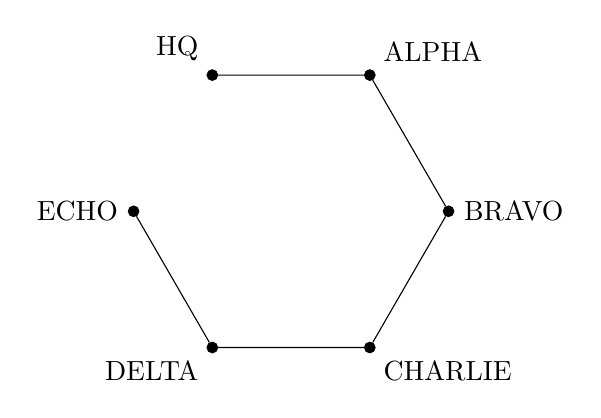
\begin{tikzpicture}[
	vertex/.style={ circle, draw, very thin, fill, inner sep=0pt, minimum size=4pt },
	vertexg/.style={ black!40!white, circle, draw, very thin, fill, inner sep=0pt, minimum size=4pt },
	vertexo/.style={ circle, draw, very thin, inner sep=0pt, minimum size=4pt }
]

% regular hexagon has interior angles of 120 degrees

\node at (0,0) (d) [vertex,label=below left:{DELTA}] {};
\node at (2,0) (c) [vertex,label=below right:{CHARLIE}] {};
\node at (3,1.73) (b) [vertex,label=right:{BRAVO}] {};
\node at (2,3.46) (a) [vertex,label=above right:{ALPHA}] {};
\node at (0,3.46) (hq) [vertex,label=above left:{HQ}] {};
\node at (-1,1.73) (e) [vertex,label=left:{ECHO}] {};
\draw (hq) to (a) to (b) to (c) to (d) to (e);

\end{tikzpicture}
